
\section{DWH Implementation}

\begin{breakbox}
\boxtitle{MOLAP:}
\newline Multi-dimensional OLAP stored in n-dimensional arrays.
\begin{center}
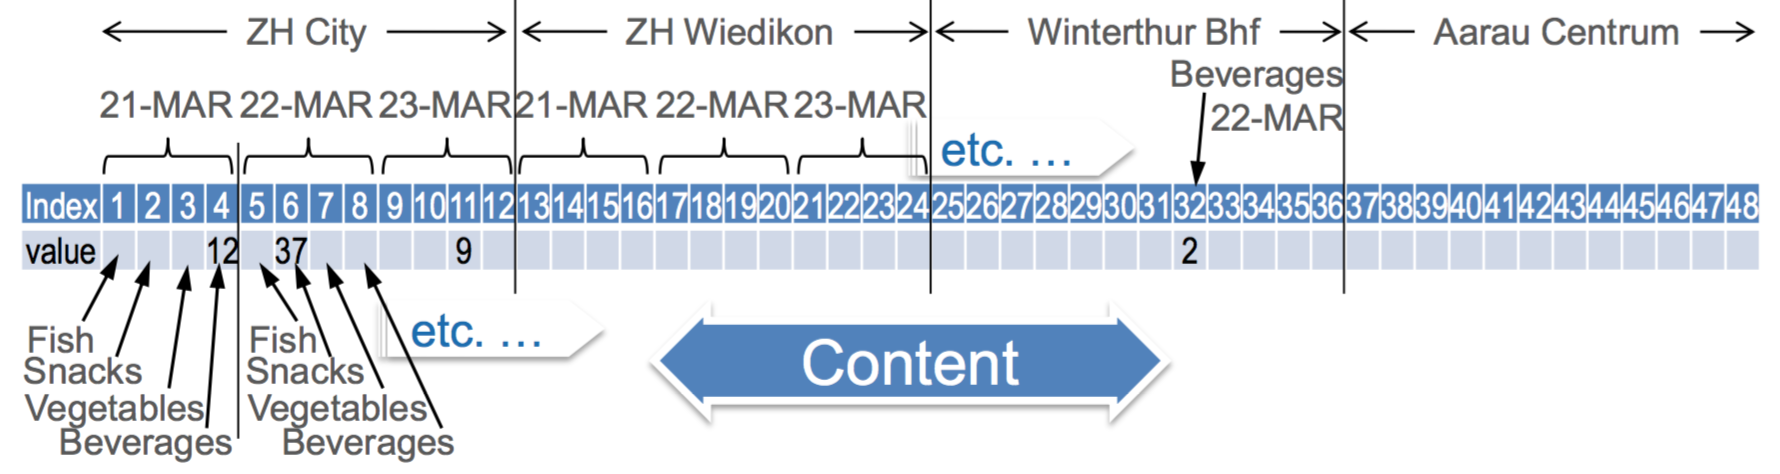
\includegraphics[width=.15\textwidth]{slides_images/molap.png}
\end{center}
Formel für storage (und query):
\begin{center}
$i_{1k} + (i_{2l-1}) \cdot |I_1| + (i_{3m}-1) \cdot |I_1| \cdot |I_2| + \cdots$,
\end{center}
mit $I_j =$ dimension $j$, $i_{jk} =$ index for $k^{th}$ element of dimension $j$.
\end{breakbox}

\begin{breakbox}
\boxtitle{Beispiel (Pages):}
\newline Folgende Tabellen und Daten sind gegeben. Die Dimensionen sind geordnet nach Shipment, Supplier, Year, Product:
\begin{center}
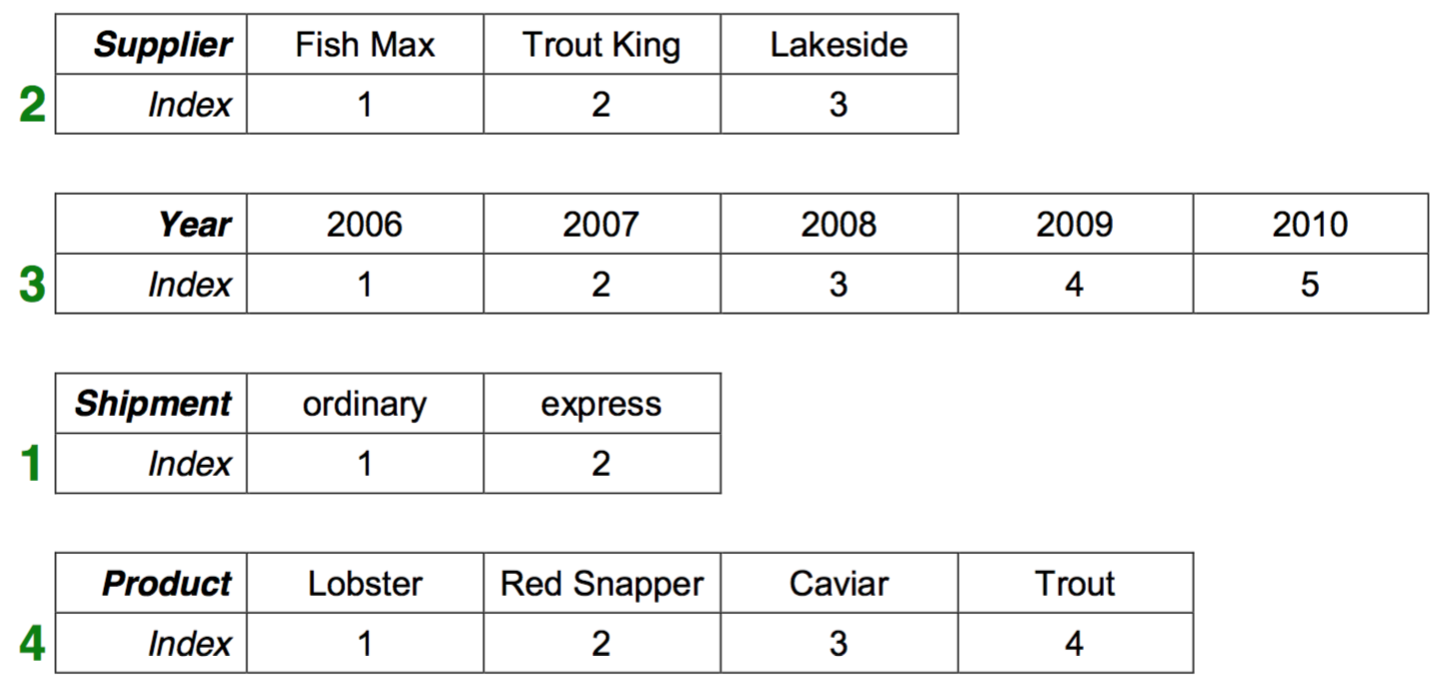
\includegraphics[width=.15\textwidth]{slides_images/molap_example.png}
\end{center}
Aufgabe: A page can hold 4 array cells.
\begin{enumerate}[label=(\alph*)]
	\item How many pages have to be loaded for a query after all sales of Lobster in 2008?
		\begin{itemize}
			\item[] All Lobster array cells adjacent (since it's last dimension in order). Lobster in 2008 spreads over 6 cells (all combinations from Supplier and Shipment dimensions). 6 / 4 = 2 pages.
		\end{itemize}
	\item How many pages have to be loaded for a query after all sales by "express" in 2008?
		\begin{itemize}
			\item[] The 2008 and express combinations spread over 5 cells (i.e. 2 pages), but there are several of those ranges , dispersed over Lobster, Red Snapper, Caviar and Trout. So 4 x 2 = 8 pages.
		\end{itemize}
\end{enumerate}
\begin{center}
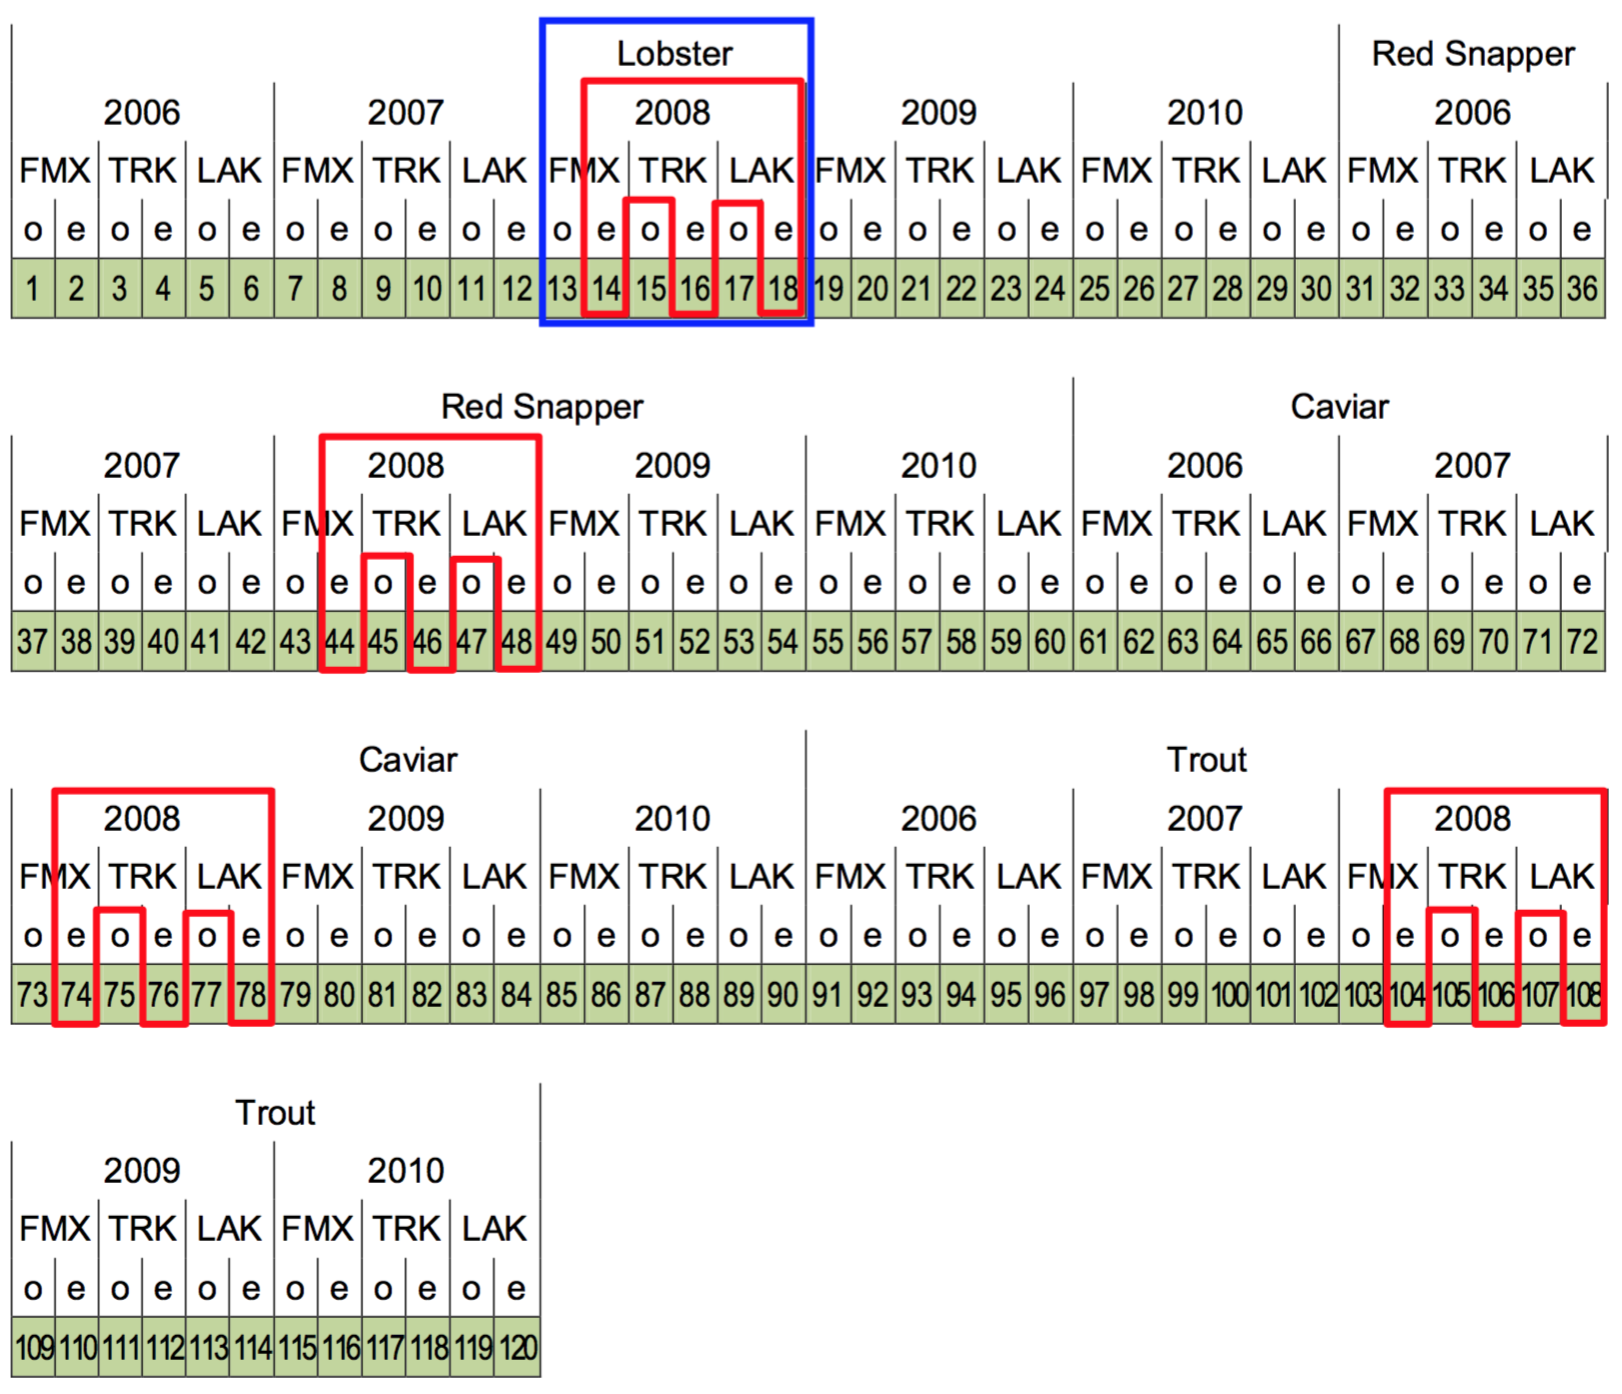
\includegraphics[width=.15\textwidth]{slides_images/molap_solution.png}
\end{center}
\end{breakbox}

\begin{breakbox}
\boxtitle{FASMI:}
\begin{itemize}
	\item \textcolor{Emerald}{F}ast: response time < 5 s, complex queries max. 20 s.
	\item \textcolor{Emerald}{A}nalysis: intuitive analytical functionality.
	\item \textcolor{Emerald}{S}hared: more than 1 user, authorization, authentication.
	\item \textcolor {Emerald}{M}ultidimensional: Multidimensional conceptual view on data.
	\item \textcolor{Emerald}{I}nformation: analysis not limited by OLAP system.
\end{itemize}
\end{breakbox}
